\documentclass[10pt,a4paper]{article}
\usepackage[T1]{fontenc}
\usepackage[utf8]{inputenc}
\usepackage{lmodern}
\usepackage[english]{babel}
\usepackage[margin=2.2cm,top=2.4cm,bottom=2.6cm]{geometry}
\usepackage{microtype}
\usepackage{amsmath,amssymb,amsthm}
\usepackage{graphicx}
\usepackage{booktabs,array}
\usepackage[font=small,labelfont=bf,labelsep=period]{caption}
\usepackage{enumitem}
\usepackage{xcolor}
\usepackage{tikz}
\usetikzlibrary{arrows.meta,positioning,fit,calc}
\usepackage[numbers,sort&compress]{natbib}
\usepackage[hidelinks]{hyperref}
\usepackage[capitalise,noabbrev]{cleveref}
\usepackage{fancyhdr}
\usepackage[section]{placeins}

\hypersetup{
  pdftitle={Zeno-free but late: ordinal event triggers with a guaranteed minimum inter-event time in master-slave Lorenz synchronisation},
  pdfauthor={Johel Padilla-Villanueva},
  pdfkeywords={event-triggered control; Zeno behaviour; minimum inter-event time; Kendall tau-b; chaos synchronisation; Lorenz system; negative result}}

\providecommand{\doi}[1]{}
\renewcommand{\doi}[1]{doi:\,\href{https://doi.org/#1}{\nolinkurl{#1}}}
\setlength{\bibsep}{2pt plus 1pt}
\renewcommand{\bibfont}{\small}
\newcommand{\te}{\tau_b^{(e)}}
\newcommand{\sgn}{\operatorname{sgn}}
\newcommand{\MIET}{\mathrm{MIET}}
\newcommand{\R}[1]{\textup{R#1}}
% generated by scripts/make_assets.py from ../results/*.csv
\newcommand{\nRuleRuns}{400}
\newcommand{\nMeasurable}{375}
\newcommand{\nViol}{0}
\newcommand{\nNoIET}{25}
\newcommand{\minIETglobal}{0.03}
\newcommand{\maxDtau}{0.20}
\newcommand{\nTies}{0}
\newcommand{\nTauNaN}{0}
\newcommand{\nDiv}{0}
\newcommand{\nRmsNaN}{0}
\newcommand{\nRunsTotal}{720}
\newcommand{\nRthreeaNoIET}{3}
\newcommand{\nRthreebNoIET}{22}
\newcommand{\medIETmin}{0.06}
\newcommand{\medIETmax}{1.51}
\newcommand{\pW}{1.9\times10^{-6}}
\newcommand{\pHolm}{7.6\times10^{-6}}
\newcommand{\maxWinsB}{0}
\newcommand{\maxWinsC}{0}
\newcommand{\nTests}{48}
\newcommand{\rmsAClean}{0.40}
\newcommand{\updAClean}{2001.0}
\newcommand{\rmsBClean}{0.70}
\newcommand{\updBClean}{774.8}
\newcommand{\rmsCClean}{1.68}
\newcommand{\updCClean}{850.7}
\newcommand{\rmsRoneClean}{12.81}
\newcommand{\updRoneClean}{183.7}
\newcommand{\rmsRtwoClean}{24.16}
\newcommand{\updRtwoClean}{15.0}
\newcommand{\rmsRthreeaClean}{20.22}
\newcommand{\updRthreeaClean}{67.4}
\newcommand{\rmsRthreebClean}{23.93}
\newcommand{\updRthreebClean}{1.0}
\newcommand{\rmsVClean}{19.31}
\newcommand{\updVClean}{209.7}
\newcommand{\rmsVAClean}{20.51}
\newcommand{\updVAClean}{2001.0}
\newcommand{\rmsPClean}{5.93}
\newcommand{\winsRonePClean}{0}
\newcommand{\updPClean}{182}
\newcommand{\rmsANoise}{1.08}
\newcommand{\updANoise}{2001.0}
\newcommand{\rmsBNoise}{1.13}
\newcommand{\updBNoise}{1636.7}
\newcommand{\rmsCNoise}{1.38}
\newcommand{\updCNoise}{992.0}
\newcommand{\rmsRoneNoise}{13.24}
\newcommand{\updRoneNoise}{168.4}
\newcommand{\rmsRtwoNoise}{21.81}
\newcommand{\updRtwoNoise}{9.3}
\newcommand{\rmsRthreeaNoise}{20.76}
\newcommand{\updRthreeaNoise}{54.4}
\newcommand{\rmsRthreebNoise}{22.27}
\newcommand{\updRthreebNoise}{3.0}
\newcommand{\rmsVNoise}{21.00}
\newcommand{\updVNoise}{170.8}
\newcommand{\rmsVANoise}{20.45}
\newcommand{\updVANoise}{2001.0}
\newcommand{\rmsPNoise}{7.94}
\newcommand{\winsRonePNoise}{1}
\newcommand{\updPNoise}{167}
\newcommand{\rmsADist}{11.97}
\newcommand{\updADist}{2001.0}
\newcommand{\rmsBDist}{8.41}
\newcommand{\updBDist}{408.6}
\newcommand{\rmsCDist}{10.01}
\newcommand{\updCDist}{960.6}
\newcommand{\rmsRoneDist}{15.47}
\newcommand{\updRoneDist}{213.1}
\newcommand{\rmsRtwoDist}{24.79}
\newcommand{\updRtwoDist}{11.3}
\newcommand{\rmsRthreeaDist}{21.84}
\newcommand{\updRthreeaDist}{79.5}
\newcommand{\rmsRthreebDist}{24.35}
\newcommand{\updRthreebDist}{11.2}
\newcommand{\rmsVDist}{19.31}
\newcommand{\updVDist}{209.7}
\newcommand{\rmsVADist}{20.51}
\newcommand{\updVADist}{2001.0}
\newcommand{\rmsPDist}{8.59}
\newcommand{\winsRonePDist}{0}
\newcommand{\updPDist}{223}
\newcommand{\rmsADrift}{10.42}
\newcommand{\updADrift}{2001.0}
\newcommand{\rmsBDrift}{11.79}
\newcommand{\updBDrift}{388.7}
\newcommand{\rmsCDrift}{11.32}
\newcommand{\updCDrift}{912.5}
\newcommand{\rmsRoneDrift}{16.57}
\newcommand{\updRoneDrift}{211.6}
\newcommand{\rmsRtwoDrift}{23.95}
\newcommand{\updRtwoDrift}{18.2}
\newcommand{\rmsRthreeaDrift}{21.28}
\newcommand{\updRthreeaDrift}{74.0}
\newcommand{\rmsRthreebDrift}{23.19}
\newcommand{\updRthreebDrift}{15.3}
\newcommand{\rmsVDrift}{19.55}
\newcommand{\updVDrift}{209.7}
\newcommand{\rmsVADrift}{21.12}
\newcommand{\updVADrift}{2001.0}
\newcommand{\rmsPDrift}{15.32}
\newcommand{\winsRonePDrift}{3}
\newcommand{\updPDrift}{223}
\newcommand{\pHfour}{1.00}
\newcommand{\VidentRMS}{20}
\newcommand{\VidentUpd}{20}
\newcommand{\winsBCClean}{20}
\newcommand{\pBCClean}{0.000}
\newcommand{\winsBCNoise}{20}
\newcommand{\pBCNoise}{0.000}
\newcommand{\winsBCDist}{17}
\newcommand{\pBCDist}{0.006}
\newcommand{\winsBCDrift}{6}
\newcommand{\pBCDrift}{0.076}

\makeatletter\newcommand{\tabinput}[1]{\@@input #1 }\makeatother

\pagestyle{fancy}\fancyhf{}
\renewcommand{\headrulewidth}{0.3pt}
\fancyhead[L]{\footnotesize Padilla-Villanueva \textbullet\ Ordinal triggers in closed-loop synchronisation}
\fancyfoot[C]{\footnotesize\thepage}
\setlength{\headheight}{13pt}

\title{\vspace{-0.6cm}\textbf{Zeno-free but late: ordinal event triggers with a guaranteed minimum inter-event time in master--slave Lorenz synchronisation}}
\author{Johel Padilla-Villanueva, DrPH\\[3pt]
\small Department of Environmental Health, Graduate School of Public Health,\\
\small Medical Sciences Campus, University of Puerto Rico, San Juan, Puerto Rico, USA\\
\small \href{mailto:joel.padilla2@upr.edu}{\nolinkurl{joel.padilla2@upr.edu}} \textbullet\ ORCID \href{https://orcid.org/0000-0002-5797-6931}{0000-0002-5797-6931}\\[2pt]
\small \doi{10.5281/zenodo.24263807}}
\date{}

\begin{document}
\maketitle
\thispagestyle{fancy}

\begin{abstract}
\noindent\textbf{Background.} Event triggers built on windowed Kendall $\tau_b$ fire when the mean absolute change $D_E$ of ordinal concordance on a fixed edge set leaves a band. For re-anchoring (\R{1}), hysteresis (\R{2}) and their $\kappa$-qualified forms (\R{3}), a sampled minimum inter-event time (MIET) has been proved and machine-checked in Lean~4, together with exact invariance of the event sequence under strictly increasing sensor distortion. Whether these guarantees yield useful closed-loop control had not been tested.
\textbf{Methods.} We inserted \R{1}, \R{2} and two $\kappa$-qualified variants (\R{3}a, \R{3}b) as the ``when to update'' layer of a two-layer master--slave Lorenz synchronisation loop with a saturated sliding-mode correction. We compared them with continuous updating, a Girard-type dynamic magnitude trigger and a naive ordinal level trigger. A rank-based correction layer (V) tested distortion invariance of the whole loop. All parameters ($W=20$, $p=1$, $\theta=0.40$, $\delta=0.20$, $\theta_\kappa=0.5$) were fixed a priori. We used 20 seeds and four sensor scenarios (clean, Gaussian noise, monotone distortion, drift), with paired Wilcoxon tests and Holm adjustment.
\textbf{Results.} The guarantees held exactly. Across \nMeasurable{} runs with a measurable inter-event time there were \nViol{} violations of the bound $2h$. The observed minimum was $3h$, and the largest one-step change of $\tau_b$ was $4/W=\maxDtau$: the bound is attained but never exceeded. The event sequence and the error of V were identical with and without distortion in all 20 seeds. Control performance, however, was poor. The magnitude trigger had lower error than every ordinal rule in every scenario and in 20 of 20 seeds (two-sided $p=\pW$, Holm-adjusted $p=\pHolm$). A periodic schedule with a comparable update budget also outperformed \R{1} (clean RMS $\rmsPClean$ vs $\rmsRoneClean$).
\textbf{Conclusion.} In this loop, a Zeno-free ordinal trigger fires too late to serve as a fine tracking trigger. It is better viewed as a structural alarm with guaranteed event separation.
\end{abstract}

\noindent\textbf{Keywords:} event-triggered control; Zeno behaviour; minimum inter-event time; Kendall $\tau_b$; ordinal concordance; chaos synchronisation; Lorenz system; negative result.

\section{Introduction}\label{sec:intro}

Event-triggered control replaces periodic actuation by updates that occur only when a state-dependent condition is met \citep{tabuada2007,heemels2012}. Its central theoretical requirement is a positive lower bound on the time between events, the minimum inter-event time (MIET). Without it a trigger can be \emph{Zeno}: it can fire infinitely often in finite time. Tabuada derived such a bound for a trigger that compares the measurement error with the state \citep{tabuada2007}. Girard introduced dynamic triggering mechanisms, with an internal filtered variable, that enlarge inter-event times while preserving stability \citep{girard2015}. Borgers and Heemels showed that several common mechanisms lose their event separation under arbitrarily small disturbances or measurement noise \citep{borgers2014}. In chaos synchronisation \citep{pecora1990}, event triggers are usually defined on the magnitude of the synchronisation error. Examples are networks of Lur'e systems \citep{liuzhou2016} and, recently, a dynamic threshold with fixed-time convergence \citep{taghavifar2026}.

A different family of triggers uses ordinal information. In the Systemic Tau programme, the signal that decides \emph{when} a system should adapt is the change of windowed Kendall $\tau_b$ \citep{kendall1938,kendall1945} on a fixed set of edges between modules. This change is summarised by the mean absolute change $D_E$, which decomposes exactly as $D_E=|\bar D_E|+C_E$ into a signed part and a cancellation part, and by the cancellation index $\kappa_E=C_E/D_E$ \citep{pv2026cancel,pv2026kappa}. Because $\tau_b$ takes values on a finite lattice and changes by bounded steps, such triggers admit a data-independent sampled MIET. In a companion preprint \citep{pv2026miet} we proved that one window shift changes $\tau_b$ by at most $4/W$. We derived MIET bounds for re-anchoring and hysteresis rules and proved that the event sequence is invariant under strictly increasing sensor distortions. This discrete core was machine-checked in Lean~4 \citep{demoura2021lean4,mathlib2020}. The same preprint reported, as a limitation, that a naive ordinal \emph{level} supervisor lost to a magnitude trigger in a two-layer synchronisation loop. The rules for which the guarantees were proved had not been tested in closed loop.

This paper performs that test. Its question is narrow: \emph{when the proved ordinal rules decide when a synchronising controller updates, do the guarantees hold in closed loop, and do they buy competitive tracking?} Our contributions are as follows.
\begin{enumerate}[leftmargin=*,itemsep=1pt]
\item A closed-loop test of rules \R{1}--\R{3} with parameters, hypotheses and statistical tests fixed a priori (\cref{sec:methods}).
\item Confirmation of the deterministic guarantees: no MIET violation in \nMeasurable{} measurable runs, and the one-step bound $4/W$ is attained but never exceeded (\cref{sec:res-miet}).
\item Confirmation that distortion invariance carries over to a whole closed loop when the correction layer is also ordinal (\cref{sec:res-inv}).
\item A clear negative result on performance. Every ordinal rule loses to a dynamic magnitude trigger in every scenario and every seed. An additional diagnostic analysis indicates that the cause is the \emph{timing} of ordinal events, not only their number (\cref{sec:res-rms,sec:periodic}).
\end{enumerate}
We report the negative result in full because it limits the role that ordinal triggers can play. In this loop they are guaranteed not to chatter, but that guarantee says nothing about whether they fire at the right time.

\section{Background: ordinal triggers and their guarantees}\label{sec:background}

We use the definitions and numbering of \citep{pv2026miet} without change. A window holds the last $W$ samples of each signal, taken with period $h$. For an edge $e=\{a,b\}$, let $n_c$ and $n_d$ be the numbers of concordant and discordant pairs among the $n_0=W(W-1)/2$ pairs of window positions, and let $n_1,n_2$ be the numbers of pairs tied in $a$ and in $b$. Then
\begin{equation}
\te=\frac{n_c-n_d}{\sqrt{(n_0-n_1)(n_0-n_2)}} .
\end{equation}
Given a baseline $B_e$ and $\Delta_e=\te-B_e$, define
\begin{equation}\label{eq:DE}
\bar D_E=\frac1{|E|}\sum_{e\in E}\Delta_e,\quad D_E=\frac1{|E|}\sum_{e\in E}|\Delta_e|,\quad C_E=\frac{2\min(S_+,S_-)}{|E|},\quad \kappa_E=\frac{C_E}{D_E}\in[0,1],
\end{equation}
where $S_+=\sum_{\Delta_e>0}\Delta_e$ and $S_-=\sum_{\Delta_e<0}|\Delta_e|$. The identity $D_E=|\bar D_E|+C_E$ holds, so $\kappa_E$ is the fraction of the total change that cancels between edges. It is near $0$ when all edges move in the same direction and near $1$ when increases and decreases balance. It is undefined when $D_E=0$.

\paragraph{Rules.} With a threshold $\theta>0$ \citep[Definition~3]{pv2026miet}:
\begin{description}[leftmargin=1.2em,style=nextline,itemsep=1pt]
\item[\R{1} (re-anchoring)] an event occurs when $D_E\ge\theta$, and the baseline is then re-anchored, $B_e\leftarrow\te(t_k)$;
\item[\R{2} (hysteresis)] $B_e$ is the fixed calibration mean. An event occurs when the trigger is armed and $D_E\ge\theta$, after which the trigger is disarmed until $D_E\le\theta-\delta$, with $\delta\in(0,\theta]$;
\item[\R{3} ($\kappa$-qualified)] \R{1} or \R{2} with the additional requirement $\kappa_E\ge\theta_\kappa$.
\end{description}
A fourth rule, which fires on $\kappa_E$ alone, can be Zeno \citep[Example~1]{pv2026miet} and is not used here.

\begin{figure}[!t]
\centering
\begin{tikzpicture}[
  font=\small, >={Stealth[length=2.2mm]},
  blk/.style={draw, rounded corners=2pt, minimum height=9mm, minimum width=25mm, align=center, fill=white},
  lay/.style={draw=black!40, dashed, rounded corners=4pt, inner sep=6pt}]
\node[blk] (m) {Master Lorenz\\$\dot x_m=f(x_m)$};
\node[blk, below=12mm of m] (s) {Slave Lorenz, mismatched\\$\dot x_s=\tilde f(x_s)+u+d(t)$};
\node[blk, right=10mm of s] (sen) {Sensor\\$y_s=\mathcal S(x_s,t)$};
\node[blk, right=22mm of sen, yshift=11mm] (trig) {Trigger layer\\[-1pt]\footnotesize A, B, C, \R{1}, \R{2}, \R{3}a, \R{3}b};
\node[blk, below=9mm of trig] (ctl) {Correction layer\\[-1pt]\footnotesize sliding mode on $e=y_s-x_m$\\[-1pt]\footnotesize (V, VA: rank law)};
\node[blk, below=8mm of ctl, minimum width=16mm] (zoh) {ZOH};
\draw[->] (s) -- (sen);
\draw[->] (sen.east) -- ++(6mm,0) |- ([yshift=-2mm]trig.west);
\draw[->] (m.east) -- ++(52mm,0) |- ([yshift=2mm]trig.west);
\draw[->] (trig) -- node[right,font=\footnotesize]{update at $t_k$} (ctl);
\draw[->] (ctl) -- (zoh);
\draw[->] (zoh.west) -| node[pos=0.3,below,font=\footnotesize]{$u(t)=u(t_k)$ for $t\in[t_k,t_{k+1})$} (s.south);
\node[lay, fit=(trig)(ctl)] (L) {};
\node[font=\footnotesize, text=black!60, anchor=south] at (L.north) {two-layer controller: when (top), how much (bottom)};
\end{tikzpicture}
\caption{Two-layer master--slave loop. The trigger layer decides when the control is recomputed. The correction layer computes the control from the measured error. Between events the control is held (zero-order hold, ZOH). The master state is read exactly; the sensor model $\mathcal S$ (clean, noise, distortion or drift) acts on the slave only.}
\label{fig:loop}
\end{figure}

\paragraph{Guarantees.} Assume no ties (assumption A0) and a window that advances by one sample per evaluation ($p=1$). Proposition~1 of \citep{pv2026miet} then gives two results. (b) One evaluation step changes each $\te$, and hence $D_E$ under a common baseline, by at most $4/W$. (c) \R{1} and \R{3}-over-\R{1} satisfy $\MIET\ge h\lceil\theta W/4\rceil$, and \R{2} and \R{3}-over-\R{2} satisfy $\MIET\ge 2h\lceil\delta W/4\rceil$, for any data and any additive noise. Proposition~5 states that if a sensor reads $y=\varphi(x)$, with $\varphi$ strictly increasing and time-invariant, then $\te$, $D_E$, $\kappa_E$ and the event sequence are identical with and without the distortion. Both results are part of the Lean~4 formalisation (repository \href{https://github.com/johelpadilla/ordinal-miet-lean}{\nolinkurl{github.com/johelpadilla/ordinal-miet-lean}}, commit \texttt{1273ec5}). The continuous-time results of \citep{pv2026miet} are proved on paper only, and its Conjecture~1 on a uniform MIET for the Lorenz flow is open; neither is used here. The present study is sampled, so it tests only the machine-checked discrete statements.

\section{Methods}\label{sec:methods}

\subsection{Two-layer synchronisation loop}\label{sec:loop}


The test bench is that of Section~8 of \citep{pv2026miet} (\cref{fig:loop}), reused without modification. All data were generated by numerical simulation. The master is the Lorenz system \citep{lorenz1963} $f(x)=(\sigma(x_2-x_1),\,x_1(\rho-x_3)-x_2,\,x_1x_2-\beta x_3)$ with $(\sigma,\rho,\beta)=(10,28,8/3)$. The slave has a $10\%$ parameter mismatch, $(11,\,30.8,\,1.1\cdot8/3)$, and a bounded disturbance $d(t)=0.5\,(\sin1.1t,\,\cos0.9t,\,\sin(0.6t+0.3))$. Both systems are integrated by the fourth-order Runge--Kutta method with step $h=0.01$ on $[0,20]$ (2000 steps). Initial states are drawn uniformly from $[-10,10]^2\times[10,30]$ by a generator seeded with $1000+\text{seed}$.

\paragraph{Correction layer.} At each event $t_k$ the control is recomputed from the measured error $e=y_s-x_m$ by a generic saturated sliding-mode law. The law uses the surface $s=e+k_1\operatorname{sig}(e)^{1/2}+k_2\operatorname{sig}(e)^{3/2}$, where $\operatorname{sig}(e)^a=\sgn(e)|e|^a$ componentwise. The control is $u=\operatorname{clip}_{[-40,40]}\big(-\eta\tanh(s/\mu)-k_{\mathrm{lin}}s\big)$, with $k_1=k_2=0.8$, $\mu=0.30$ and $k_{\mathrm{lin}}=8$. The adaptive gain starts at $\eta=8$ and is updated at each event by $\eta\leftarrow\min\{\eta+h\gamma\sum_i|s_i|,\,60\}$, with $\gamma=1.5$. The control is held constant between events. This law is a generic re-implementation inspired by \citep{taghavifar2026}; it is not the controller of that paper.

\paragraph{Sensor scenarios.} Only the slave is measured; the master state is available exactly. There are four scenarios. \emph{Clean}: $y_s=x_s$. \emph{Noise}: $y_s=x_s+\nu$, with $\nu\sim\mathcal N(0,0.8^2)$ independent per channel and step, from a generator seeded with $50000+\text{seed}$. \emph{Distortion}: $y_s=\varphi(x_s)=x_s+10\tanh(x_s/15)$ componentwise, which is strictly increasing with $\varphi'\ge1$. \emph{Drift}: $y_s=x_s+0.25\,t$. For a given seed, all methods share the same initial conditions and noise realisation.

\subsection{Trigger and correction policies}\label{sec:policies}

Ordinal quantities use the three paired edges $E=\{(x_{m,1},y_{s,1}),(x_{m,2},y_{s,2}),(x_{m,3},y_{s,3})\}$, so $|E|=3$, and a window of $W=20$ samples of master state and slave measurement. Every method starts with one update at $t=0$.
\begin{description}[leftmargin=1.2em,style=nextline,itemsep=1pt]
\item[A, continuous] The control is recomputed at every step (reference).
\item[B, dynamic magnitude trigger] A Girard-type rule \citep{girard2015}. Let $\varepsilon=e-e(t_k)$ and define the slack $\sigma_B\|e\|+\epsilon_0-\|\varepsilon\|$. An internal variable is updated as $\eta_d\leftarrow\max\{0,\eta_d+h(-\lambda\eta_d+\text{slack})\}$, and an event occurs when $\eta_d+\theta_B\,\text{slack}\le0$. The parameters are $\sigma_B=0.5$, $\epsilon_0=0.6$, $\lambda=2$, $\theta_B=1$ and $\eta_d(0)=0.5$. These values were chosen in preliminary simulations of the original bench so that B made fewer updates than A without losing synchronisation in the clean case. They are not taken from \citep{taghavifar2026}.
\item[C, naive ordinal level trigger] The original ordinal supervisor of \citep{pv2026miet}. It is evaluated every second sample ($p=2$) and fires whenever the mean of the three $\te$ is below $0.95$, with neither re-anchoring nor hysteresis.
\item[\R{1}] The re-anchoring rule on $D_E$, evaluated at every sample ($p=1$) once the window is full. The initial anchor is the $\tau_b$ of the first full window, without an event.
\item[\R{2}] The hysteresis rule, with the fixed calibration baseline $B_e$ of \cref{sec:calib}.
\item[\R{3}a, \R{3}b] \R{1} and \R{2}, respectively, with the additional requirement $\kappa_E\ge\theta_\kappa$. An undefined $\kappa_E$ ($D_E=0$) does not qualify.
\item[V, ordinal correction] The \R{1} trigger combined with a rank-based correction. For each channel $i$, let $r_s$ and $r_m$ be the mid-ranks of the current slave measurement and of the current master value within their own windows, scaled to $[0,1]$. The control is $u_i=-40\,(r_s-r_m)$. Ranks are invariant under strictly increasing maps, so both \emph{when} and \emph{how much} the loop acts are invariant under distortion. This gives an exact prediction for Proposition~5 at the level of the whole loop.
\item[VA] The same rank law, updated at every step. This secondary diagnostic separates the effect of the trigger from that of the rank law.
\end{description}
If any $\te$ were undefined (a window with all values tied), the evaluation would not fire. Windows with ties, which would violate A0, were counted.

\subsection{Parameters and calibration}\label{sec:calib}

The thresholds were fixed a priori by the following rule and were not tuned. $\theta=8/W=0.40$ is the smallest multiple of the one-step bound $4/W$ that makes the \R{1} guarantee non-trivial, $\lceil\theta W/4\rceil=2$ evaluations. We set $\delta=\theta/2=0.20$, the ratio used in the numerical check of \citep{pv2026miet}. We set $\theta_\kappa=0.5$, so that at least half of the change must be internal cancellation. With these values every rule has the same guaranteed bound,
\begin{equation}\label{eq:bound}
\MIET_{\R1,\,\R3\mathrm a,\,\mathrm V}\ge h\lceil\theta W/4\rceil=2h=0.02,\qquad \MIET_{\R2,\,\R3\mathrm b}\ge 2h\lceil\delta W/4\rceil=2h=0.02 .
\end{equation}
Rules \R{2} and \R{3}b need the \emph{calibration mean} of $\te$ as their baseline $B_e$, as required by Definition~2 of \citep{pv2026miet}. It was estimated separately for each scenario from the continuous policy A on calibration seeds 100--104, which are disjoint from the evaluation seeds 0--19. The estimate is the per-edge mean of $\te$, evaluated at every sample with $t\in[6,20]$ (7005 windows per scenario). The resulting values were $(0.8835,0.8821,0.9466)$ for clean sensors, $(0.6427,0.6483,0.7728)$ for noise, $(0.5084,0.3403,0.5630)$ for distortion and $(0.7337,0.5335,0.7786)$ for drift.

\subsection{Outcomes, hypotheses and statistics}\label{sec:stats}

The primary performance outcome is the root-mean-square \emph{true} synchronisation error $\big(\frac1N\sum\|x_s-x_m\|^2\big)^{1/2}$ over $t\in[6,20]$, which discards the transient. The event outcomes are the number of control updates on $[0,20]$, including the initial one; the minimum and median inter-event time (IET) of each run; and the largest one-step change $\max|\te(t_{j+1})-\te(t_j)|$ over consecutive tie-free evaluations. A run with at most one event has no IET and cannot test a MIET bound. Such runs are reported separately and counted neither as compliant nor as violations.

The study tested four hypotheses:
\begin{itemize}[leftmargin=2.6em,itemsep=1pt]
\item[\textbf{H1}] (deterministic) every \R{} rule respects its bound \eqref{eq:bound} in all runs, and the one-step change of $\tau_b$ never exceeds $4/W=0.2$;
\item[\textbf{H2}] the \R{} rules have a larger median IET than C;
\item[\textbf{H3}] \R{1}--\R{3} differ from B in true RMS error (two-sided; no direction was predicted);
\item[\textbf{H4}] under distortion, V has lower RMS than B (one-sided), and V's RMS is identical with clean and distorted sensors for every seed.
\end{itemize}
RMS errors were compared with the exact two-sided paired Wilcoxon signed-rank test \citep{wilcoxon1945} over the 20 seeds, computed with SciPy \citep{virtanen2020scipy}. Each new method was compared with B and with C in each scenario (\nTests{} tests). The $p$-values were adjusted by Holm's step-down procedure within each family, defined as one method against one reference across the four scenarios. With $n=20$ and all signs equal, the smallest attainable two-sided exact $p$ is $2^{-19}\approx1.9\times10^{-6}$. This caps the strength of evidence that the design can report. H4 used a one-sided paired Wilcoxon test. Computations used NumPy \citep{harris2020numpy}, SciPy and Matplotlib \citep{hunter2007matplotlib}.

\subsection{Verification of the implementation}\label{sec:qc}
The implementation was verified in four ways. (i) Policies A, B and C reproduced the 240 results of the earlier bench \citep{pv2026miet} exactly; the clean RMS of A was $\rmsAClean$, as in that bench. (ii) The new simulation loop, run in condition A, reproduced the original A in all 80 runs. (iii) An independent re-implementation of $D_E$, $\kappa_E$ and the rules, sharing no code with the main implementation, re-derived exactly the event sequences of all 400 rule runs from the computed $\tau_b$ series. (iv) Repeating the full set of simulations from scratch gave identical results.

\section{Results}\label{sec:results}

There were no divergences and no undefined RMS values in the $\nRunsTotal$ runs (9 methods $\times$ 4 scenarios $\times$ 20 seeds). No evaluated window contained ties, so A0 held throughout, and no $\tau_b$ was undefined.

\subsection{The MIET guarantees hold exactly (H1, H2)}\label{sec:res-miet}

\begin{figure}[tbp]
\centering
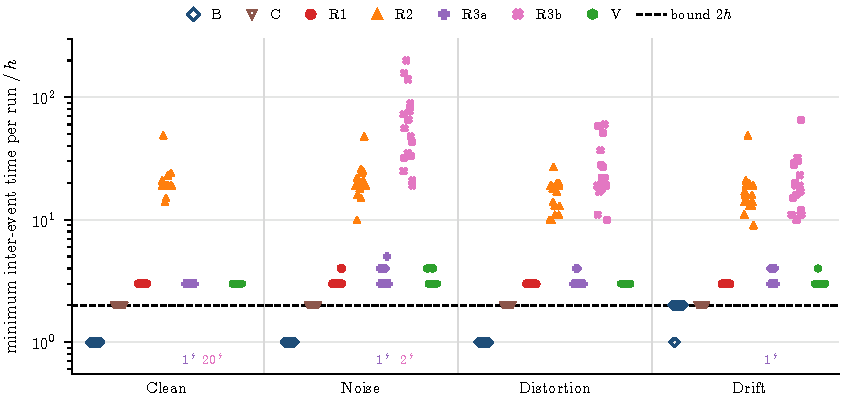
\includegraphics[width=\linewidth]{figures/fig_miet_bound.pdf}
\caption{Observed minimum inter-event time per run, in units of the sampling period $h$, against the guaranteed bound of Proposition~1(c) of \citep{pv2026miet}. The dashed line is the bound, $2h$ for every rule with the parameters of \cref{sec:calib}. Each marker is one of the 20 seeds, with horizontal jitter; the vertical axis is logarithmic. Open markers are the baselines B and C, which carry no ordinal guarantee; filled markers are the rules. Numbers marked $\dagger$ count runs with at most one event, which have no inter-event time. This happens for \R{3}b in all 20 clean runs and in 2 noise runs, and for \R{3}a in one run in each of three scenarios.}
\label{fig:miet}
\end{figure}

\begin{table}[tbp]
\centering\small
\caption{Event statistics of the ordinal rules (20 seeds per cell). Bound: guaranteed MIET from \eqref{eq:bound}. Min IET: minimum over the 20 runs. Median IET: median of the per-run medians. Comply, No IET and Violate: numbers of runs whose minimum IET is at least the bound, that have at most one event, and whose minimum IET is below the bound. Max $|\Delta\tau_b|$: largest one-step change of $\te$ over tie-free consecutive evaluations, to be compared with $4/W=0.20$. Times are in model time units ($h=0.01$).}
\label{tab:miet}
\setlength{\tabcolsep}{5pt}
\begin{tabular}{@{}llccccccc@{}}
\toprule
Rule & Scenario & Bound & Min IET & Median IET & Comply & No IET & Violate & Max $|\Delta\tau_b|$\\
\midrule
\tabinput{generated/tab_miet.tex}
\bottomrule
\end{tabular}
\end{table}

H1 was confirmed without exception (\cref{fig:miet,tab:miet}). In total, \nRuleRuns{} runs were governed by an \R{} trigger (\R{1}, \R{2}, \R{3}a, \R{3}b and V). Of these, \nMeasurable{} had at least two events, and all of them respected the bound $2h=0.02$; none violated it. The other \nNoIET{} runs had a single, initial update (\nRthreebNoIET{} for \R{3}b and \nRthreeaNoIET{} for \R{3}a). The smallest inter-event time observed under any rule was $\minIETglobal=3h$. The largest one-step change of $\tau_b$ was $\maxDtau$, which equals $4/W$ to machine precision. The bound of Proposition~1(b) is therefore attained in closed loop but never exceeded, as it must be. Under A0 the numerator $n_c-n_d$ changes by at most $2(W-1)=38$ per step, and $38/n_0=38/190=0.2$.

H2 was also confirmed. The medians of the per-run median IETs of the rules ranged from $\medIETmin$ to $\medIETmax$. C had a median IET of $0.02$, its evaluation step, in every scenario. B, which has no ordinal guarantee, reached the sampling period $h$ (one step) in every scenario (\cref{fig:miet}). Under \R{2} and \R{3}b the hysteresis band produced median spacings of $0.71$ to $1.51$, that is, roughly 35 to 75 times the bound.

\subsection{Distortion invariance carries over to the whole loop (H4, invariance part)}\label{sec:res-inv}

Under the monotone distortion $\varphi(x)=x+10\tanh(x/15)$, policy V produced exactly the same RMS error and the same number of updates as with clean sensors in \VidentRMS{} of 20 seeds (\cref{fig:diag}b). This is what Proposition~5 predicts when both layers depend on the data only through ranks. VA, which applies the same rank law at every step, was likewise identical across the two scenarios. The invariance is exact and holds by construction. It does not imply good control, however. The directional part of H4 failed: under distortion V had an RMS of $\rmsVDist$, worse than B ($\rmsBDist$) in every seed (one-sided $p=\pHfour$).

\subsection{Tracking error: every ordinal rule loses (H3)}\label{sec:res-rms}

\begin{table}[tbp]
\centering\small
\caption{True RMS synchronisation error over $t\in[6,20]$ (mean $\pm$ SD over 20 seeds) and mean number of control updates on $[0,20]$, including the initial update. Bold: lowest mean RMS in each scenario among all policies except A. \R{3}b with clean sensors never fired after $t=0$; its row therefore shows the error of a loop that holds its initial control for the whole run.}
\label{tab:rms}
\setlength{\tabcolsep}{3.5pt}
\begin{tabular}{@{}lcccccccc@{}}
\toprule
& \multicolumn{2}{c}{Clean} & \multicolumn{2}{c}{Noise} & \multicolumn{2}{c}{Distortion} & \multicolumn{2}{c}{Drift}\\
\cmidrule(lr){2-3}\cmidrule(lr){4-5}\cmidrule(lr){6-7}\cmidrule(l){8-9}
Policy & RMS & Upd. & RMS & Upd. & RMS & Upd. & RMS & Upd.\\
\midrule
\tabinput{generated/tab_rms.tex}
\bottomrule
\end{tabular}
\end{table}

\begin{figure}[tbp]
\centering
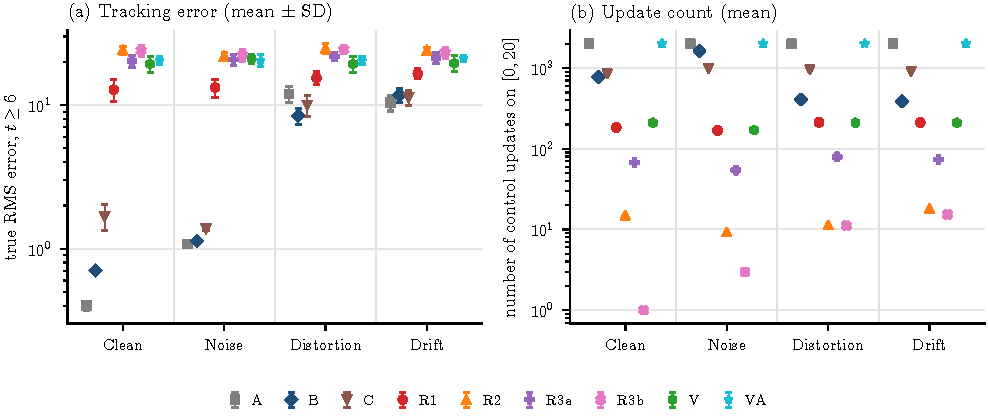
\includegraphics[width=\linewidth]{figures/fig_rms_updates.pdf}
\caption{(a) True RMS synchronisation error ($t\ge6$; mean $\pm$ SD over 20 seeds) and (b) mean number of control updates, for all policies and scenarios. Both vertical axes are logarithmic. The ordinal rules (\R{1}--\R{3}b) and the rank policies (V, VA) have mean errors between \rmsRoneClean{} and \rmsRtwoDist{}. With clean or noisy sensors this is an order of magnitude above B and C. These policies made between \updRthreebClean{} and \updRoneDist{} updates on average, apart from VA, which updates at every step.}
\label{fig:rms}
\end{figure}

The performance comparison is unambiguous and negative (\cref{tab:rms,fig:rms}). With clean sensors the dynamic magnitude trigger B reached an RMS error of $\rmsBClean$ with $\updBClean$ updates. The best ordinal rule, \R{1}, reached $\rmsRoneClean$ with $\updRoneClean$ updates. \R{2} ($\rmsRtwoClean$), \R{3}a ($\rmsRthreeaClean$) and \R{3}b ($\rmsRthreebClean$) were at or near the level of the loop that holds its initial control (\R{3}b with clean sensors, a single update). The same ordering held with noise, distortion and drift. For every new method (\R{1}, \R{2}, \R{3}a, \R{3}b, V and VA) and every scenario, B had the lower error in 20 of 20 seeds. Each of these 24 comparisons gave the smallest attainable two-sided exact $p=\pW$, or $p=\pHolm$ after Holm adjustment. The same was true against the naive ordinal trigger C. Across all \nTests{} tests, the new method had the lower error in \maxWinsB{} of 20 seeds against B and in \maxWinsC{} of 20 against C. H3 is therefore answered. In this loop the proved ordinal rules lose by a large margin to the magnitude trigger, and also to the unguaranteed ordinal level trigger.

Two secondary observations concern the baselines. First, with distorted or drifting sensors even continuous updating (A) performed poorly ($\rmsADist$ and $\rmsADrift$), and under distortion A was worse than B. The error measured through the distorted or drifting sensor is a biased estimate of the true error. Any magnitude law that drives the measured error to zero therefore leaves a structural offset, and updating more often does not remove it. Second, B had lower error than C in \winsBCClean{}, \winsBCNoise{} and \winsBCDist{} of 20 seeds with clean, noisy and distorted sensors, respectively. Under drift it did so in only \winsBCDrift{} of 20 seeds (two-sided $p=\pBCDrift$, not distinguishable), which reproduces the earlier report \citep{pv2026miet}.

\subsection{Diagnostic analysis: the problem is timing, not only budget}\label{sec:periodic}

\begin{figure}[tbp]
\centering
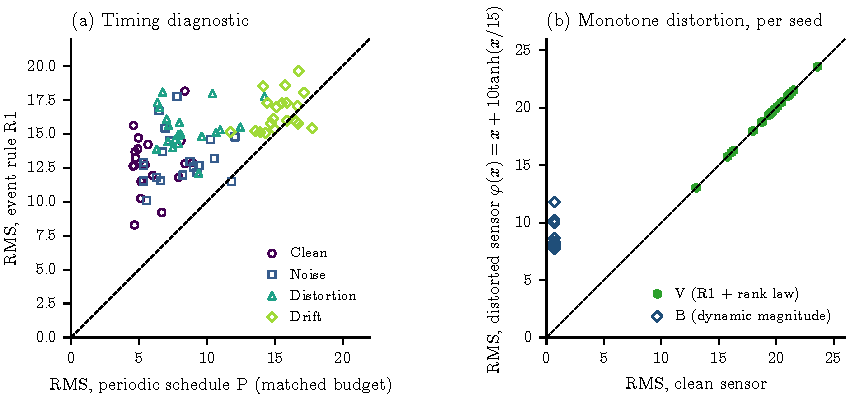
\includegraphics[width=\linewidth]{figures/fig_diagnostics.pdf}
\caption{(a) Timing diagnostic. Per-seed RMS of rule \R{1} against a periodic schedule P whose period gives approximately the same number of updates as \R{1} in each scenario (\cref{tab:periodic}). Points above the dashed identity line are seeds in which the periodic schedule had lower error. (b) Per-seed RMS with clean versus distorted sensors. V (filled hexagons) lies exactly on the identity line, as predicted by Proposition~5; B (open diamonds) does not.}
\label{fig:diag}
\end{figure}

\begin{table}[tbp]
\centering\small
\caption{Periodic schedule P versus rule \R{1} (additional diagnostic analysis, outside the primary hypotheses). The period, in steps of $h$, was $\mathrm{round}\big(2000/(\bar n_{\R1}-1)\big)$, where $\bar n_{\R1}$ is the mean number of \R{1} updates in the scenario. RMS: mean $\pm$ SD over 20 seeds. ``\R{1} better'': number of seeds in which \R{1} had lower RMS. $p$: two-sided exact paired Wilcoxon test, not adjusted for multiplicity.}
\label{tab:periodic}
\begin{tabular}{@{}lccccccc@{}}
\toprule
Scenario & Period & Upd.\ P & Upd.\ \R{1} & RMS P & RMS \R{1} & \R{1} better & $p$\\
\midrule
\tabinput{generated/tab_periodic.tex}
\bottomrule
\end{tabular}
\end{table}

A low update count alone could explain the gap to B, since with clean sensors \R{1} updates about a quarter as often as B. To separate the number of updates from their timing, we compared \R{1} with a periodic schedule P with about the same number of updates. This additional diagnostic analysis lies outside the four primary hypotheses (\cref{tab:periodic,fig:diag}a). P beat \R{1} in all four scenarios. With clean sensors P had a slightly smaller budget than \R{1} ($\updPClean$ vs $\updRoneClean$ updates) and reached an RMS of $\rmsPClean$ versus $\rmsRoneClean$; \R{1} was better in \winsRonePClean{} of 20 seeds. With noise the result was similar (\R{1} better in \winsRonePNoise{} of 20). Rounding the period gave P about $5\%$ more updates than \R{1} under distortion and drift, so those two comparisons are less tightly matched; under drift the gap was small ($\rmsPDrift$ vs $\rmsRoneDrift$). With a comparable or smaller budget, then, regularly spaced updates tracked better than updates placed by the ordinal trigger. The \R{1} events are not merely too few; they come at the wrong times.

\section{Discussion}\label{sec:discussion}

\paragraph{What was confirmed.} The discrete guarantees of \citep{pv2026miet} survived a closed loop with chaotic dynamics, parameter mismatch, a disturbance, noise, distortion and drift. No rule fired faster than the bound allows. The one-step bound $4/W$ was reached exactly, which shows that it is tight and not merely safe. With an ordinal correction layer, the invariance of Proposition~5 extended from the event sequence to the whole closed-loop trajectory. Magnitude triggers do not have these properties for free: B reached the sampling floor $h$, and its error changed with the distortion (\cref{fig:diag}b).

\paragraph{Why the ordinal rules lose.} We offer an interpretation that is consistent with the data but was not itself tested. Windowed $\tau_b$ between master and slave measures whether the two signals rise and fall together over the last $W$ samples, which here span $0.19$ time units. While the slave is close to the master, the orders coincide and $\tau_b$ stays near its anchor. A change of $D_E$ by $\theta=0.4$, on a scale where one sample moves $\tau_b$ by at most $0.2$, requires a substantial fraction of the $190$ window pairs to reverse. That happens only once synchronisation has already degraded. The high-gain sliding law, in contrast, needs frequent updates to hold synchronisation: with clean sensors A used 2001 updates and B used $\updBClean$. The ordinal trigger is therefore reactive by construction. It reports that the order structure has changed, and that change is a late symptom of lost synchronisation. The periodic diagnostic supports this reading: about the same number of updates at fixed times did better, so the weakness lies in \emph{when} the rule fires.

The $\kappa$ qualification made matters worse. When synchronisation is lost, the three edge correlations tend to fall together. The $\Delta_e$ then share a sign and $\kappa_E$ is close to $0$. A rule that requires $\kappa_E\ge0.5$ vetoes exactly these coherent changes, which are the informative ones for tracking. This account is consistent with \R{3}a making roughly a third as many updates as \R{1} (\cref{tab:rms}) and with \R{3}b never firing after $t=0$ with clean sensors. We did not, however, record $\kappa_E$ at rejected candidate events, so the mechanism should be read as a hypothesis. The hysteresis rules have a further failure mode in tracking. After an event they stay disarmed until $D_E$ returns within $\theta-\delta$ of a fixed baseline, and this may not happen while the control remains frozen.

\paragraph{What ordinal triggers are good for.} These results do not weaken the guarantees; they delimit what the guarantees mean. A MIET bound excludes chattering. It does not certify that the trigger is informative for a given control objective. Ordinal triggers with re-anchoring or hysteresis suit roles that need a certified, distortion-invariant and Zeno-free signal and can tolerate delay. Examples are a supervisory alarm for structural reorganisation, a gate that releases adaptation or repair, and a monitor that runs on uncalibrated monotone sensors. They are not substitutes for a magnitude trigger in a high-gain tracking loop. This agrees with the earlier negative result for the naive level supervisor \citep{pv2026miet} and sharpens it. That result could have been attributed to the absence of re-anchoring and hysteresis; the present one cannot.

\paragraph{Relation to magnitude-based event triggering.} The ordinal bound is a counting argument on the order lattice and holds for any data, including data with additive noise. Magnitude triggers obtain their bounds from Lipschitz and input-to-state stability estimates of the closed loop \citep{tabuada2007,girard2015}, and such bounds can be fragile under noise \citep{borgers2014}. This study confirmed the robustness of the ordinal bound and also made its price visible. Because the rule ignores magnitude, it cannot react to a growing error until the error has disturbed the ordering.

\section{Limitations}\label{sec:limits}
\begin{itemize}[leftmargin=*,itemsep=2pt]
\item \emph{Single configuration.} We tested one window ($W=20$), one set of thresholds ($\theta=0.40$, $\delta=0.20$, $\theta_\kappa=0.5$), one controller and one horizon ($T=20$). No other values were tried. This avoids tuning on the outcome, but it leaves the dependence on the parameters unknown. With these values the guaranteed bound ($2h$) is small. A larger $\theta W$ would give stronger guarantees and, presumably, even later events.
\item \emph{Evaluation rate.} The new rules were evaluated at every sample ($p=1$), as Proposition~1(c) requires in its simplest form. The original trigger C was evaluated every second sample ($p=2$). Comparisons with C therefore mix the effect of the rule with that of the evaluation rate.
\item \emph{Baseline calibration.} The calibration mean $B_e$ for \R{2} and \R{3}b was estimated per scenario from the continuous policy A on separate seeds. Other choices are possible and would change these rules. For example, $B_e=1$ would make every $\Delta_e\le0$, hence $\kappa_E\equiv0$, so \R{3}b could never fire.
\item \emph{Baseline tuning.} The parameters of B came from preliminary simulations of the original bench, in which B was required to keep synchronisation with clean sensors. By design, the ordinal rules received no comparable tuning. This favours B. It cannot, however, account for differences of the observed size, nor for the loss to the periodic schedule.
\item \emph{Error bias under distortion and drift.} The master is read exactly while the slave passes through the sensor. The measured error, $\varphi(x_s)-x_m$ or $x_s+0.25t-x_m$, is therefore biased for every magnitude law, including A and B. Proposition~5 concerns the event sequence and says nothing about this bias.
\item \emph{Generic controller.} The sliding-mode law is a re-implementation inspired by \citep{taghavifar2026}, not that paper's controller. The comparison is therefore not a test of that work.
\item \emph{Statistics.} With 20 seeds the exact Wilcoxon test cannot report $p<1.9\times10^{-6}$, so the $p$-values reflect a floor and not the effect size; the RMS differences give the effect sizes. The periodic comparison is an additional diagnostic analysis outside the primary hypotheses; its $p$-values are not adjusted, and its update budget is matched only approximately.
\item \emph{Simulation only.} No physical or experimental data were used. A sampled simulation also cannot test the continuous-time results or Conjecture~1 of \citep{pv2026miet}.
\end{itemize}

\section{Conclusion}\label{sec:conclusion}

Ordinal event triggers with re-anchoring or hysteresis kept their proved, machine-checked guarantees in a closed chaotic loop. Their inter-event times never fell below the bound, the one-step bound was reached exactly, and distortion invariance extended to the whole trajectory when the correction layer was ordinal. As update policies for a high-gain synchronising controller, however, they were clearly worse than a dynamic magnitude trigger and than a naive ordinal level trigger. An additional diagnostic comparison showed that they were also worse than a periodic schedule with a comparable budget. A guarantee against Zeno behaviour is not a guarantee of good control. In this loop the ordinal trigger is best regarded as a Zeno-free, distortion-invariant structural alarm, not as a fine tracking trigger. Natural next steps are a systematic sweep over $W$ and $\theta$, a record of $\kappa_E$ at rejected candidate events, and a test in a supervisory role, such as gating adaptation or repair, where late but certified events may be exactly what is required.

\section*{Data and code availability}\label{sec:data}
{\sloppy The simulation code, the simulated data and the source of this article are openly available at \href{https://github.com/johelpadilla/ordinal-triggers-lorenz-sync}{\nolinkurl{github.com/johelpadilla/ordinal-triggers-lorenz-sync}} and archived at Zenodo, \doi{10.5281/zenodo.24263807}. The companion preprint is available at \doi{10.5281/zenodo.24260444} (concept \doi{10.5281/zenodo.24227492}). The Lean~4 formalisation is available at \href{https://github.com/johelpadilla/ordinal-miet-lean}{\nolinkurl{github.com/johelpadilla/ordinal-miet-lean}} (commit \texttt{1273ec587ec288b19bf1ffcf98e9ca6ba7c522d4}).\par}

\section*{Declarations}
\paragraph{Funding.} This work received no specific funding.
\paragraph{Competing interests.} The author declares no competing interests. The study evaluates statistics and trigger rules that the author introduced in earlier work.
\paragraph{Declaration of generative AI and AI-assisted technologies.} During the preparation of this work the author used Grok (xAI) to assist with writing the simulation and analysis code and with the preparation and editing of the text. After using this tool, the author reviewed and edited the content as needed and takes full responsibility for the content of the article.
\paragraph{Ethics.} Not applicable; no human or animal data were used.

\bibliographystyle{unsrtnat}
\bibliography{refs}

\end{document}
